\documentclass[11pt]{article}
\usepackage{tocloft}
\usepackage{graphicx}
\usepackage{calc}
\usepackage{amssymb}
\usepackage{color}
\usepackage{array}
\usepackage[sc]{mathpazo}
\usepackage{url}
\usepackage[final]{pdfpages}
\usepackage{amsmath}

%\linespread{1.05}
\oddsidemargin=0pt
\evensidemargin=0pt
\textwidth=6.5in
\topmargin=0pt
\headheight=0pt
\headsep=0pt
\textheight=9in
% EXPERIMENTAL
%\parindent=0pt
%\parskip=3pt
\setlength{\parindent}{0cm}
\newcommand\secfont{\fontfamily{cmss}\selectfont}%\textwidth 5.5truein
\newcommand\pifheading[1]{{\secfont\textbf{#1}:}}
%\oddsidemargin -0.40truein
%\textheight 8.0truein
%\topmargin -0.25truein
\def\lo{
\mathrel{\raise.3ex\hbox{$<$}\mkern-14mu\lower0.6ex\hbox{$\sim$}}
}
\def\hi{
\mathrel{\raise.3ex\hbox{$>$}\mkern-14mu\lower0.6ex\hbox{$\sim$}}
}

\textwidth = 6.6 in
\textheight = 9.1 in
\oddsidemargin = -0.05 in
\evensidemargin = +0.05 in
\topmargin = -.1 in
\headheight = 0.0 in
\headsep = 0.0 in
\parskip = 0.06in
\newcommand\registered{{\ooalign{\hfil\raise .00ex\hbox{\scriptsize R}\hfil\crcr\mathhexbox20D}}}

%% Define a new 'leo' style for the package that will use a smaller font.
\makeatletter
\def\url@leostyle{%
  \@ifundefined{selectfont}{\def\UrlFont{\sf}}{\def\UrlFont{\small\ttfamily}}}
\makeatother
%% Now actually use the newly defined style.
\urlstyle{leostyle}

%\pagestyle{empty}
%\includeonly{previous,proposal_references}
%\includeonly{proposal_references}
%\includeonly{previous}

% TOC

\begin{document}
%%%%%%%%%%%%%%%%%%%%%%%%%%%%%%%%%%%%%%%%%%%%%%%%%%%%%%%%%%%%%%%%%%%%%
\begin{center}
\textbf{\Large
AST101: Our Corner of the Universe \\
\vspace*{0.1cm}
Lab 7: Spectroscopy Prelab 
}
\end{center}

\vspace*{0.5cm}

{\Large Name:}\vspace*{0.5cm}\\\hrule
{\Large Student number (SUID):}\vspace*{0.5cm}\\\hrule
{\Large Lab section:}\vspace*{0.5cm}\\\hrule
\vspace*{0.5cm}

%%%%%%%%%%%%%%%%%%%%%%%%%%%%%%%%%%%%%%%%%%%%%%%%%%%%%%%%%%%%%%%%%%%%%
\section{Introduction}

In the next few labs, we'll be studying the properties of light -- specifically, how different objects interact with different colors of light, and how we can learn about the composition and temperature of objects by examining their wavelength.

Wavelength is associated with color. For instance, the shortest-wavelength light that we can see appears blue or purple, and the longest-wavelength light that we can see appears red. But there are other ``colors'' of light -- other wavelengths -- that we 
can't see. For instance, x-rays have very short wavelength and radio waves have very long wavelength, but they are both types of light. This range of wavelengths is called the {\it electromagnetic spectrum} and is sometimes visualized like this:

\begin{center}
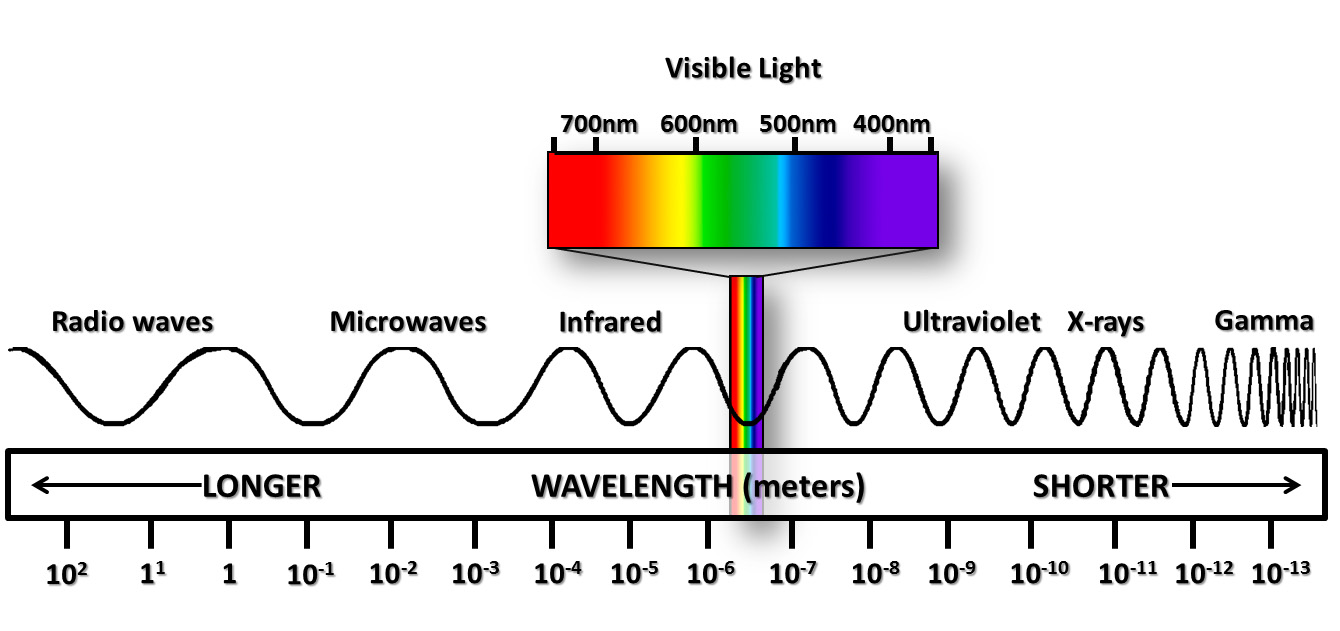
\includegraphics[width=4in]{linear-spectrum.jpg}
\end{center}

For this prelab, we'll focus mostly on those colors that we can see.\footnote{One of the difficulties in this business is the very limited way that our eyes see color. You may have learned that there are ``three primary colors'' -- red, green, and blue. However, these colors are not special; they are simply the {\it colors our eyes
can detect}. When we are exposed to yellow light, for instance, its wavelength lies between red and green, and thus stimulates both the red and green receptors in our eyes. Our brain says ``Aha! This must be yellow!'' So our eyes are not the best tool around
for perceiving color: we can't tell, for instance, whether we are looking at a mix of red and green light, or whether we are looking at actual yellow light. In class and lab, we'll talk about some instruments that let us do better than our eyes. But, for this prelab,
there may be multiple plausible answers, because of how our eyes work. That's okay.}

Since a great way to visualize things is to make a graph, we often make graphs of ``how much light'' vs. ``color of light''. Later we'll label color with numerical values for wavelength, but for now we'll just use the names of colors. The light reflected from the 
greenish-yellow grass outside, for instance, might look like this:


\begin{center}
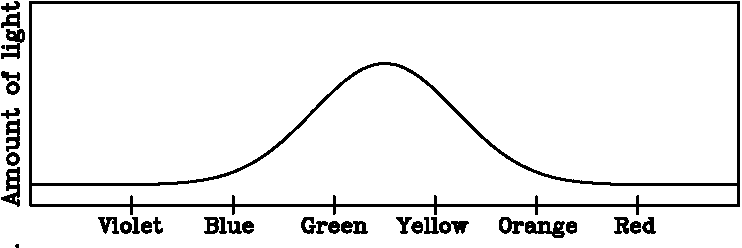
\includegraphics[width=4in]{green-yellow-crop.pdf}
\end{center}

You could read this as ``lots of green and yellow light, and a little bit of other colors''. 

Note that light that appears white is a fairly equal mixture of all colors of visible light; you know this because white light can be split into a rainbow (containing all those colors) in various ways.

\section{Drawing spectra}

Draw spectra that depict the colors of the following:

\begin{center}

\large

The sky with no clouds:

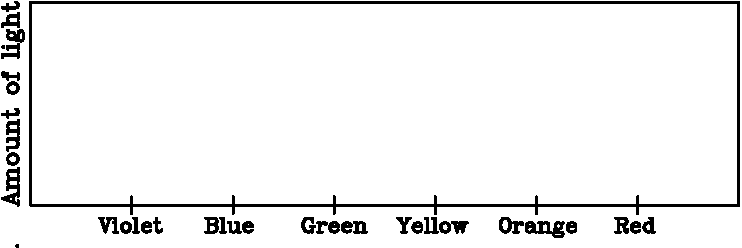
\includegraphics[width=4in]{blank-spectrum-crop.pdf}

\bigskip

The color shirt you're wearing right now:

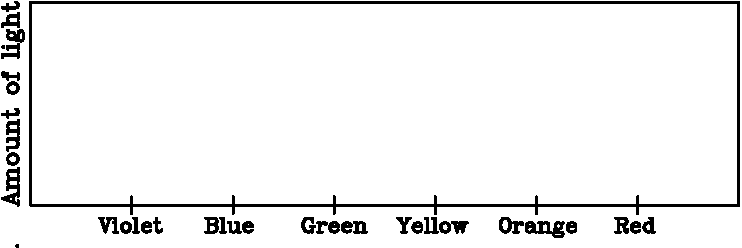
\includegraphics[width=4in]{blank-spectrum-crop.pdf}
\bigskip
\newpage
The colors of a sunset:

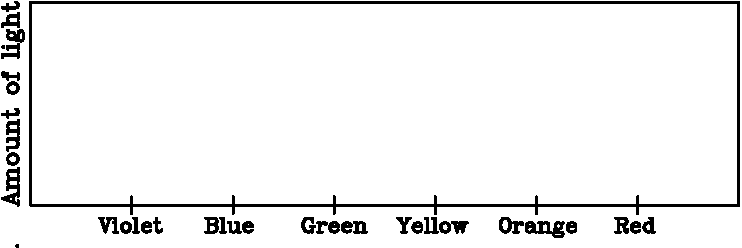
\includegraphics[width=4in]{blank-spectrum-crop.pdf}
\bigskip

\end{center}
\section{Spectra from hot objects}

One of the most common sources of light in the Universe is the glow of hot objects, like stars. This phenomenon is called {\it incandescence}. 
Light from incandescence tends to produce broad spectra: the Sun doesn't just emit a single color of light, it emits light of many different 
nearby wavelengths. The hotter it is, the shorter the wavelength it emits.

As you may know, if you heat an object up, it will first appear red (``red hot''), then begin to turn orange, yellow, and white, as the colors of light 
that it emits shift to shorter and shorter wavelengths.

Given this, draw spectra that depict the colors of the following. (They should obviously reflect your experience with these objects!)

\begin{center}

\large

The Sun, which has a temperature of about 5000 degrees C:

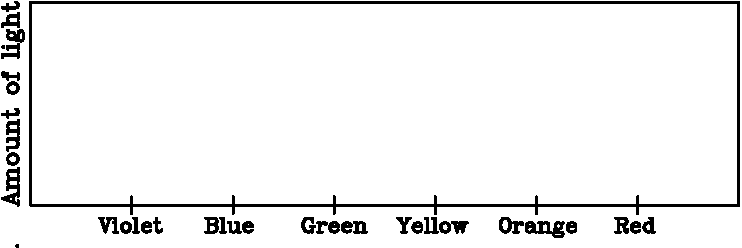
\includegraphics[width=4in]{blank-spectrum-crop.pdf}

\bigskip

A candle flame, which has a temperature of about 1200 degrees C:

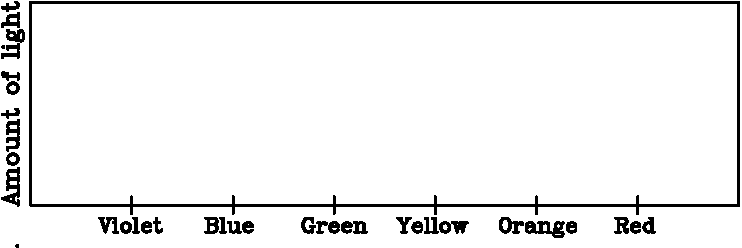
\includegraphics[width=4in]{blank-spectrum-crop.pdf}
\bigskip
\newpage
The burner of a stove, heated enough that it just barely begins to glow (around 600 degrees C)

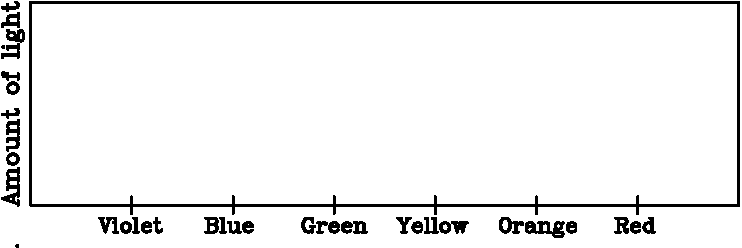
\includegraphics[width=4in]{blank-spectrum-crop.pdf}
\bigskip

\end{center}

Imagine the last example -- the stove burner, heated up enough that it just starts to glow. Imagine that you turn the power off so that it cools down to
450 degrees, so you can no longer see it glow. Is it still emitting light? If not, explain why not. If so, draw its spectrum below.

\begin{center}

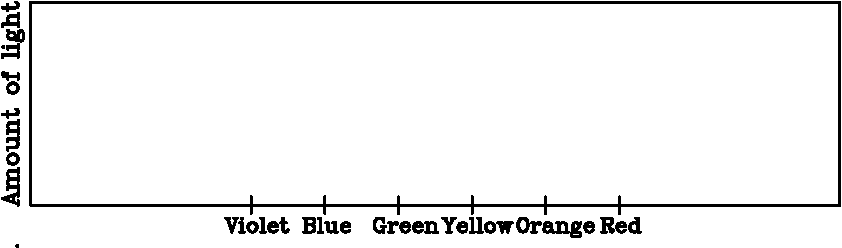
\includegraphics[width=4in]{broad-spectrum-crop.pdf}

\end{center}


\end{document}
